\chapter{Исследовательская часть}

\section{Технические характеристики}
Технические характеристики устройства, на котором выполнялись замеры по времени, представлены далее.
\begin{itemize}
	\item Процессор: AMD Ryzen 5 5500U\,--\,2.10 ГГц;
	\item Оперативная память: 16 ГБайт;
	\item Операционная система: Windows 10 Pro 64-разрядная система версии 22H2.
\end{itemize}

При замерах времени ноутбук был включен в сеть электропитания и был нагружен только системными приложениями.

\section{Демонстрация работы программы}
На рисунке \ref{img:demonstration} представлена демонстрация работы разработанного ПО.  
\begin{figure}[h]
	\centering
	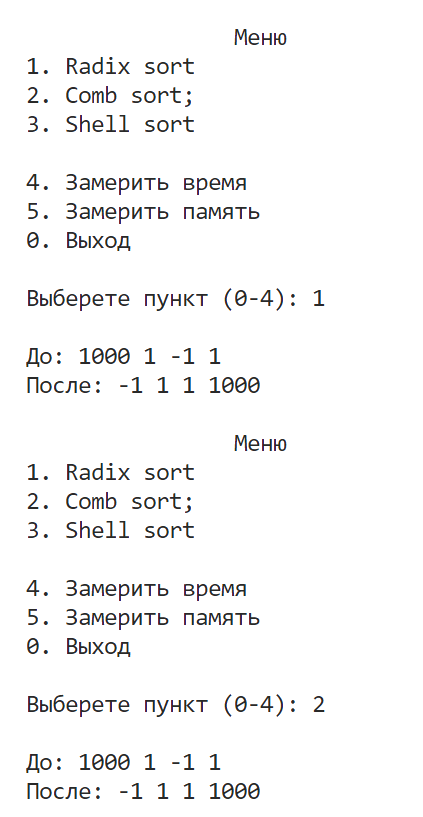
\includegraphics[height=0.3\textheight]{img/prog_work.png}
	\caption{Демонстрация работы программы}
	\label{img:demonstration}
\end{figure}

\section{Затраты по времени выполнения реализаций алгоритмов}
Все замеры проводились на массивах, размером от 1000 до 10000 с шагом 1000. 
Поскольку замеры по времени имеют некоторую погрешность, замеры производились 100 раз, а затем вычислялось среднее арифметическое значение.

Результаты замеров времени приведены в таблицах \ref{tbl:time_asc}--\ref{tbl:time_rand}.

На рисунках \ref{plt:time_01}--\ref{plt:time_03} приведены графики зависимостей работы алгоритмов от размеров матриц.

\begin{table}[h!]
    \caption{Результаты замеров времени (данные упорядочены по возрастанию)}
    \label{tbl:time_asc}
	\centering
		\begin{tabular}{|c|c|c|c|}
			\hline
			& \multicolumn{3}{c|}{Время, мкс} \\ \cline{2-4}
			Размер массива & Поразрядная & Расческой & Шелла
			\csvreader{tables/time_asc.csv}{}
			{\\\hline \csvcoli & \csvcolii & \csvcoliii & \csvcoliv} 
			\\
			\hline
		\end{tabular}
\end{table}

\begin{table}[h!]
    \caption{Результаты замеров времени (данные упорядочены по убыванию)}
    \label{tbl:time_desc}
	\centering
		\begin{tabular}{|c|c|c|c|}
			\hline
			& \multicolumn{3}{c|}{Время, мкс} \\ \cline{2-4}
			Размер массива & Поразрядная & Расческой & Шелла
			\csvreader{tables/time_des.csv}{}
			{\\\hline \csvcoli & \csvcolii & \csvcoliii & \csvcoliv} 
			\\
			\hline
		\end{tabular}
\end{table}

\begin{table}[h!]
    \caption{Результаты замеров времени (данные не отсортированы)}
    \label{tbl:time_rand}
	\centering
		\begin{tabular}{|c|c|c|c|}
			\hline
			& \multicolumn{3}{c|}{Время, мкс} \\ \cline{2-4}
			Размер массива & Поразрядная & Расческой & Шелла
			\csvreader{tables/time_rand.csv}{}
			{\\\hline \csvcoli & \csvcolii & \csvcoliii & \csvcoliv}  
			\\
			\hline
		\end{tabular}
\end{table}

\clearpage

\begin{figure}[H]
	\centering
	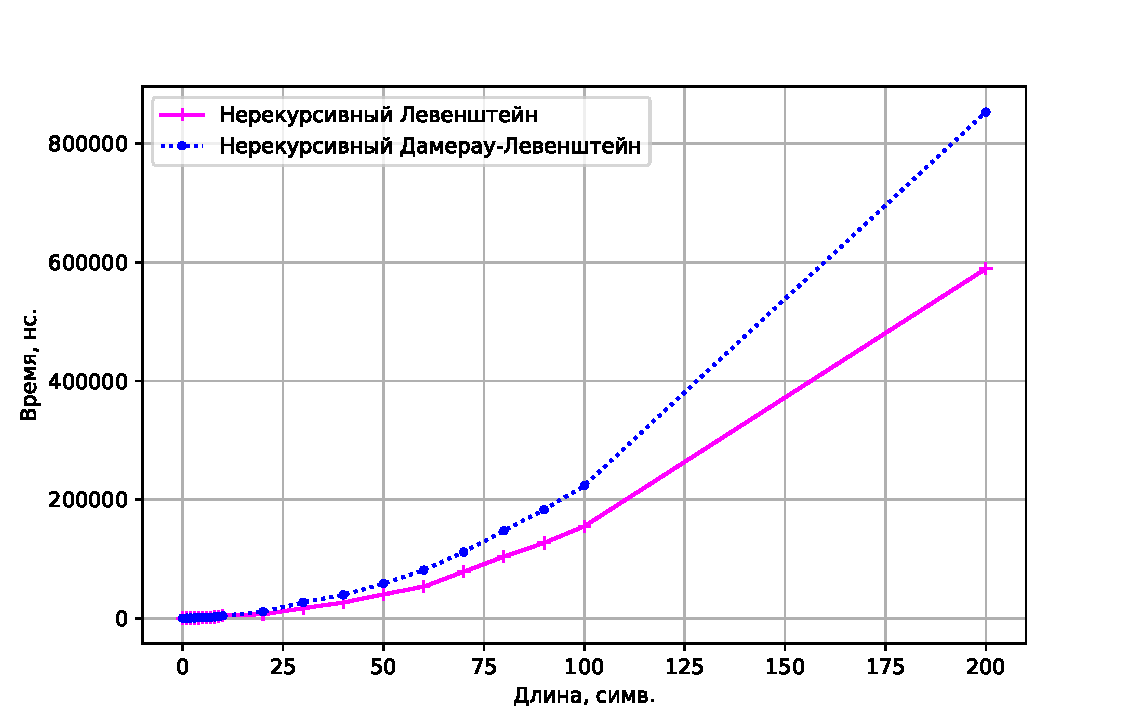
\includegraphics[height=0.4\textheight, page=1]{img/figures.pdf}
	\caption{Сравнение по времени алгоритмов сортировок на упорядоченном по возрастанию массиве}
	\label{plt:time_01}
\end{figure}


\begin{figure}[H]
	\centering
	\includegraphics[height=0.4\textheight, page=2]{img/figures.pdf}
	\caption{Сравнение по времени алгоритмов сортировок на упорядоченном по убыванию массиве}
	\label{plt:time_02}
\end{figure}

\clearpage

\begin{figure}[H]
	\centering
	\includegraphics[height=0.4\textheight, page=3]{img/figures.pdf}
	\caption{Сравнение по времени алгоритмов сортировок на случайно заполненном массиве}
	\label{plt:time_03}
\end{figure}

На упорядоченных данных сортировка расческой работает дольше всех, поскольку алгоритм расходует лишнее время на выполнение ненужных операций, что делает его неэффективным в этом случае.
На этих же данных сортировка Шелла работает быстрее расчески, что обусловлено размером шага, с которым алгоритм идет по массиву.
Порязрядная сортировка работате быстрее из всех перечисленных~--- это связано с тем, что ее сложность не зависит от порядка элементов в массиве.

На произвольных данных

\section{Затраты по памяти реализаций алгоритмов}

Затраты по памяти прдеставлены в таблице~\ref{tbl:mem_rand} и на рисунке~\ref{plt:time_04}.

\begin{table}[h!]
    \caption{Результаты замеров памяти}
    \label{tbl:mem_rand}
	\centering
		\begin{tabular}{|c|c|c|c|}
			\hline
			& \multicolumn{3}{c|}{Память, байт} \\ \cline{2-4}
			Размер массива & Поразрядная & Расческой & Шелла
			\csvreader{tables/memory.csv}{}
			{\\\hline \csvcoli & \csvcolii & \csvcoliii & \csvcoliv} 
			\\
			\hline
		\end{tabular}
\end{table}

\begin{figure}[H]
	\centering
	\includegraphics[height=0.4\textheight, page=4]{img/figures.pdf}
	\caption{Сравнение по времени алгоритмов сортировок на случайно заполненном массиве}
	\label{plt:time_04}
\end{figure}

Сортировки Шелла и расческой требуют меньше памяти, чем поразрядная, так как для последней необходимо создавать дополнительные массивы.

\section*{Вывод}
